\documentclass[a4paper,10pt]{article}
\usepackage{amsmath}
\usepackage{graphicx}
\usepackage{geometry}
\geometry{a4paper, left=2cm, right=2cm, top=1.5cm, bottom=3cm}
\usepackage{caption}
\usepackage{subcaption}
\usepackage{hyperref}
\usepackage{natbib}
\usepackage{algorithm}
\usepackage{algpseudocode}
\usepackage{times}
\usepackage{xcolor}
\usepackage{fancyhdr}
\usepackage{etoolbox}
\usepackage{setspace} 


% Header and footer configuration
\fancyhf{}
\fancyhead[R]{
\includegraphics[width=0.25\textwidth]{rennesLogo.jpg}}
\fancyfoot[L]{Research Project}
\fancyfoot[C]{University of Rennes - M1 Cybersecurity Track}
\fancyfoot[R]{\thepage}
\setlength{\headheight}{15mm}
\pagestyle{fancy}

% Patch commands for header and footer color
\newcommand{\headrulecolor}[1]{\patchcmd{\headrule}{\hrule}{\color{#1}\hrule}{}{}}
\newcommand{\footrulecolor}[1]{\patchcmd{\footrule}{\hrule}{\color{#1}\hrule}{}{}}

\renewcommand{\headrulewidth}{1pt}
\renewcommand{\footrulewidth}{1pt}
\headrulecolor{black!100}
\footrulecolor{black!100}

\bibliographystyle{apalike}

\begin{document}

\noindent 
\begin{center}
\textbf{{\Large How do Pre-treatments Influence Side-Channel Attacks?}} \\
\vspace{10pt}
\textbf{Spring Semester 2024 - M1 Cybersecurity Track}
\end{center}

\noindent 
\textbf{Authors: Thomas Feuilletin, Fabien Guihard, Ulysse Le Huitouze, Evenn Resnais, Théo Mainguet} \textit{(University of Rennes, France).}\\

\noindent 
\textbf{Research Supervisor: Damien Marion} \textit{(University of Rennes, France)}, \textbf{Benoît Gérard} \textit{(ANSSI, France)} \\
\\
\noindent 
\textbf{KEYWORDS:} SCA - Side-Channel Attack. CPA - Correlation Power Analysis. LRA - Linear Regression Analysis. Pre-processing - Pre-treatments. AES - Advanced Encryption Standard. Traces - Side-Channel measurements.

\begin{spacing}{0.82}
    \tableofcontents
\end{spacing}
\newpage

\noindent 
\textbf{ABSTRACT:} The effectiveness of side-channel attacks has been a critical topic in cybersecurity since their emergence in the late 1990s. 
SCAs exploit physical measurements like power consumption to extract cryptographic keys, and while many studies have focused on direct attack methodologies, the impact of preprocessing techniques on the efficiency of SCAs remains underexplored. 
This research investigates the influence of various preprocessing methods on the success rates of Correlation Power Analysis and Linear Regression Analysis attacks. By analyzing simulated power traces from both software and hardware implementations of the AES algorithm, we evaluate preprocessing methods including raw, squared, absolute value, centered, and standardized traces.
Our findings reveal that our current preprocessing methods don't significantly improve attack effectiveness. 
As the number of traces increases, the impact of preprocessing diminishes even more, with all methods converging towards accurate key identification. This study highlights the potential of preprocessing to refine SCA strategies and suggests future integration of deep learning techniques to further enhance preprocessing and attack methodologies.

\section{Introduction}
The exploration of Side Channel Attacks has extremely evolved since their beginning in the late 1990s, connecting the theoretical and practical aspects of cybersecurity.\\
\newline
A side-channel attack is a type of attack that uses physical measurements to break a cryptosystem.
Various physical information sources are possible in SCAs, such as:
\begin{itemize}
    \item \textit{Power consumption}: The most common source, where variations in electrical power usage are analyzed to infer cryptographic keys.

    \item \textit{Electromagnetic emissions}: These are emissions from a device during computation that can be captured and analyzed.

    \item \textit{Acoustic signals}: Sounds emitted by electronic devices or their components, like capacitors and coils, which can vary depending on the operations performed.
    
    \item \textit{Thermal imaging}: Measures the heat emitted during cryptographic operations, which can differ based on the data being processed.

\end{itemize}
In this project, we use power consumption sources and attempt to analyze a less charted but crucial aspect of SCA: the impact of preprocessing on the efficiency of attacks. \\
\newline
Preprocessing in data analysis refers to the initial steps taken to prepare raw data for further processing or analysis. 
The aim is to improve the quality of data and make it suitable for extracting meaningful insights and building predictive models.\\
\\
While numerous studies, among which the works by \cite{moussaaliabdellatif:emse-01490735} on Correlation Power Analysis or the one by \cite{Fu2017LinearRS} on Linear Regression Analysis, focus on direct attack methodologies, 
there remains a significant gap in the literature concerning the impact of preprocessing techniques on improving SCA outcomes. \\
\newline
Our work was initially inspired by studying the fundamental insights offered by the paper 'Behind the Scene of Side Channel Attacks'
by \cite{paper1}. This paper primarily introduced us to understanding LRA, CPA, and the role of preprocessing in enhancing the effectiveness of side-channel attacks.
\\ \\
In the context of our project, "traces" refers to the measurable physical outputs or activities recorded from a cryptographic device during the operation of encrypting or decrypting data.
For us, these traces include power consumption profiles. The idea is that each trace captures specific aspects of the device's behavior that can inadvertently leak sensitive information about the cryptographic process.
\\ \\
Our study refers to side-channel measurements as traces, thus the measurement complexity is stated as number of traces, one of the most common metrics in the side-channel field.
\\ \\
By analyzing the nuances and implications of preprocessing raw power traces, our study aims to shed light on potential improvements in SCA effectiveness, a topic brely addressed in current scholarly discussion. 
This gap signifies not just an opportunity for academic contribution but also a step toward refining practical attack strategies that could potentially improve the parameters of cybersecurity measures.\\
\newline
Drawing upon a structured exploration of CPA and LRA, this report is designed to document our journey from conceptual foundation to hands-on exploration and analytical synthesis.

\section{Literature Review}
In our preliminary exploration of SCAs and their methodologies, we delved into the paper "Behind the Scene of Side Channel Attacks".
For us, this paper bascially served as a foundational text in understanding the theoretical approaches to SCAs and the practical challenges related to them.
\\
\newline
As introduced earlier, SCAs exploit the physical leakages from cryptographic devices, such as power consumption or electromagnetic emissions, to extract secret keys used within cryptographic algorithms. 
Among various techniques discussed in the paper, it elaborates on CPA and LRA from a theoretical and practical perspective, having a direct link for us to the overall focus of the project on the impact of preprocessing.

\subsection{Correlation Power Analysis Basics}
\subsubsection{Overview}
Correlation Power Analysis is a form of side-channel attack that exploits statistical correlations between the known plaintext (or ciphertext), the key and the power consumption measurements of a cryptographic device. 
SCAs target the implementation of cryptographic algorithms rather than their theoretical weakness. 

\subsubsection{Pearson’s Correlation Coefficient}
By using Pearson's correlation coefficient, CPA quantifies the linear relationship between the predicted power consumption based on hypothetical guesses and the actual power measurements observed. \\
\\
This approach is effective in identifying the correct cryptographic keys by focusing on those instances where the correlation is maximized, indicating a high likelihood of correct guesswork. 
\subsubsection{Power Models}
The strength of CPA lies in its ability to work with a simple model of power consumption (like the Hamming weight or distance models), which reduces the complexity of the analysis while maintaining high effectiveness in extracting keys from many types of cryptographic implementations.

\subsubsection{Importance of S-Box Output}
The following pseudocode presented in algorithm (\ref{algo1}) outlines a basic implementation of CPA targeting AES, where the correlation analysis focuses on the power models derived from the AES S-box operations, a crucial component in the AES encryption process. 
\\
\\
In our context, the interest in the output of the S-box arises because this step in the AES algorithm significantly influences the power consumption of the cryptographic device during encryption, largely due to the non-linearity of the S-box, which introduces complexity in the encryption process.
CPA actually exploits the fact that the power consumption during the computation of the S-box values depends on the specific data being processed.

\subsubsection{Algorithm Implementation}
The pseudocode presented in algortihm \ref{algo1} encapsulates the steps involved in setting up the analysis environment, computing power models for each key candidate, and evaluating the correlation to determine the most likely key.

\begin{algorithm}
    \caption{CPA Basic Implementation on AES}
    \label{algo1}
    \begin{algorithmic}
    \State $NB\_CANDIDATES \gets 256$
    \State $NB\_TRACES \gets 1000$ \\
    \Function{ComputePowerModel}{$plain\_texts$, $func$}
        \State Initialize $res$ with zeros
        \For{$k = 0$ to $NB\_CANDIDATES - 1$}
            \State $res[k] \gets \text{apply } func \text{ on } Sbox[plain\_texts \oplus k]$
        \EndFor
        \State \Return $res$
    \EndFunction \\
    \Function{FindKey}{$index$, $power\_models$, $traces$}
        \State Initialize correlation array $res$
        \For{$k = 0$ to $NB\_CANDIDATES - 1$}
            \State Calculate correlation for each key hypothesis
            \State Store the result in $res[k]$
        \EndFor
        \State \Return $res$
    \EndFunction\\
    \State Load plain text and traces
    \State $power\_models \gets \Call{ComputePowerModel}{plain\_text, power\_model\_w}$
    \State $key\_correlations \gets \Call{FindKey}{0, power\_models, traces}$
    \State Analyze $key\_correlations$ and identify key candidates
    \end{algorithmic}
\end{algorithm}

\newpage 

\subsection{Linear Regression Analysis Basics}
\subsubsection{Overview}

Linear Regression Analysis in the context of SCAs was a bit more complex for us to understand but yet providing an interesting method. LRA seeks to model the relationship between the power consumption data points and the hypothetical leakage models linearly.
\subsubsection{Methodology}
This method (\ref{algo2}) involves constructing a linear model that predicts the device's power consumption as a linear function of the secret key and observed data (like plaintexts or ciphertexts). The coefficients of this linear model (which include the secret key) are estimated using least squares to minimize the error between the predicted and observed power consumptions.

\subsubsection{Advantages of LRA}
The main advantage of LRA over CPA is its robustness in its ability to provide a more detailed understanding of the leakage characteristics of the cryptographic device.

\subsubsection{Computational Complexity}
However, LRA is computationally more demanding compared to CPA due to several key reasons related to the complexity and nature of the computations involved.\\
LRA requires constructing and solving linear regression models, which involve extensive matrix operations. 
Specifically, for each key hypothesis, LRA computes a regression matrix  $M_k$ and its associated coefficients $B_k$ using the pseudoinverse pinv($M_k^T M_k$) $M_k^T L$.

\subsubsection{Matrix Computations}
These matrix computations, especially the inversion or pseudoinversion, are computationally intensive, particularly as the size of the matrices grows with the number of traces and data points.  
LRA must perform these matrix operations iteratively for each key hypothesis (256 in the case of AES) and for each trace, resulting in a significant computational load. The need to handle and process large datasets for each hypothesis increases the computational burden compared to CPA, which performs simpler statistical correlations.

\subsubsection{Algorithm Implementation}
\begin{algorithm}
    \caption{LRA Basic Implementation on AES}
    \label{algo2}
    \begin{algorithmic}
    \State $NB\_CANDIDATES \gets 256$
    \State $NB\_TRACES \gets 1000$ \\
    \Function{LRAFindKey}{$data$, $leakage$}
        \State Compute unique data points and initialize matrices
        \For{$k = 0$ to $NB\_CANDIDATES - 1$}
            \State Compute regression matrix $M_k$ for each key hypothesis
            \State Compute $B_k$ using pinv($M_k^T M_k$) $M_k^T L$
            \State Compute the Mean Squared Error (MSE) and store the best candidate
        \EndFor
        \State \Return Best candidate based on the least error
    \EndFunction \\
    \State Load plain text and traces
    \State $best\_candidate \gets \Call{LRAFindKey}{plain\_text, traces}$
    \State Evaluate the performance of each key candidate
    \end{algorithmic}
\end{algorithm}

\section{Power Models}
In our analysis, we implement both Hamming Weight and Hamming Distance as power models to extract insights into cryptographic processes. 
These models help us deducing crucial information such as secret keys by analyzing the effects of data manipulations on these metrics.

\subsection{Hamming Weight}
The Hamming Weight of a binary string is defined as the count of '1's in the sequence. 
It represents the number of symbols that differ from the zero-symbol of the binary alphabet. 
This measure is particularly useful in estimating power consumption, as many cryptographic devices show a correlation between power consumption and the Hamming Weight of the data being processed \cite{Fan2022}.
\\ \\
In the context of CPA, Hamming Weight is especially useful because it allows us to make consistent predictions 
about the power consumption associated with each possible key guess. 
By modeling the expected power consumption as the sum of the Hamming Weights of the intermediate values generated 
during cryptographic computation (such as after an S-box lookup), 
we can accumulate these predicted values over multiple encryption cycles. This accumulated data forms a robust statistical 
basis for correlating the predicted power consumption with the actual power measurements. 
This correlation basically helps in identifying the correct cryptographic key by highlighting the key guess that best matches the power consumption pattern observed during encryption.
\\ \\
This approach leverages the simplicity of calculating Hamming Weight and its direct relationship with power usage, making it the easiest method in CPA for efficiently processing and analyzing large datasets.
\subsection{Hamming Distance}
The Hamming Distance between two strings of equal length is the total number of positions at which the corresponding symbols differ. 
It quantifies the required number of bit-flips needed to transform one string into another, or the minimum number of errors that could have changed one string into the other. This metric is valuable in scenarios where power consumption is significantly influenced by the transition of data states.

\section{Accumulative Correlation Power Analysis}
\subsection{Overview}
The following CPA (\ref{algo3}) method utilizes Pearson's correlation coefficient in an accumulative manner, processing side-channel attack data incrementally to manage memory and computation efficiently.\\
Our method evaluates the relationship between the collected side-channel data (traces) and various hypothetical scenarios based on key guesses. 

\subsection{Methodology}
The algorithm we implemented strategically accumulates sums and squares of both the trace data and the model outputs, iterating over all possible key bytes and guesses
\\
\newline
We are here analyzing side-channel traces represented as $X^{d}_{q}$, 
where \(d\) represents the number of data points in each trace and \(q\) is the number of traces. 

\subsection{Iterative Calculations}
Our analysis is structured around iterative calculations, with outer loops running over all traces and nested loops computing over key bytes \(B\)
 (16, representing the typical number of bytes in a cryptographic key block) and guess values (256, corresponding to all possible values a single byte can take, ranging from 0 to 255).

\paragraph{Accumulators Initialization}
Firstly, we initiate accumulators for $x$ ($acc_{x}$), for $x^2$ ($acc_{x^2}$), for $y$ ($acc_{y}$), for $y^2$ ($acc_{y^2}$), and for $xy$ ($acc_{xy}$).
These accumulators will hold the sums of the respective values across all traces.
The outer loop over $q$ processes traces incrementally, avoiding the loading of all traces into memory at once. Then, we add the values of each trace and its square to the accumulators $acc_x$ and $acc_{x^2}$ respectively.

\paragraph{Key Byte and Guess Calculations}
For each key byte $B$ (16 in total) and each possible guess (256 in total), we perform the following:
\begin{itemize}
    \item Update $acc_y[B, \text{Guess}]$ by adding the output of a model function, which is dependent on the byte $B$, the guess value, and the input.

    \item Similarly, update $acc_{y^2}[B, \text{Guess}]$ with the square of the model output.

    \item Update $acc_{xy}[B, \text{Guess}]$ with the product of the model output and the trace value for the current $q$.

\end{itemize}

\subsection{Algorithm Implementation}

\begin{algorithm}
\begin{spacing}{0.85}
    \caption{Iterative Calculation of Accumulative Statistics for CPA}
    \label{algo3}
    \begin{algorithmic}
    \Require $X^{d}_{q}$ \Comment{Side-channel traces where $d$ is data points per trace and $q$ is total number of traces}
    \Ensure Pearson's correlation coefficients for each key guess
    \State Initialize $acc_x$, $acc_{x^2}$, $acc_y$, $acc_{y^2}$, $acc_{xy}$
    \For{$q$}
        \State $\text{acc\_x} \gets \text{acc\_x} + X^{d}_{q}$
        \State $\text{acc\_x}^2 \gets \text{acc\_x}^2 + (X^{d}_{q})^2$
        \For{$B = 1$ to $16$} \Comment{For each byte of the key}
            \For{$\text{Guess} = 0$ to $255$} \Comment{For each possible key guess}
                \State $\text{model\_output} \gets \text{model}(B, \text{Guess}, \text{input})$
                \State $\text{acc\_y}[B, \text{Guess}] \gets \text{acc\_y}[B, \text{Guess}] + \text{model\_output}$
                \State $\text{acc\_y}^2[B, \text{Guess}] \gets \text{acc\_y}^2[B, \text{Guess}] + \text{model\_output}^2$
                \State $\text{acc\_xy}[B, \text{Guess}] \gets \text{acc\_xy}[B, \text{Guess}] + \text{model\_output} \times X^{d}_{q}$
            \EndFor
        \EndFor
    \EndFor
    \State Compute $m_x = \frac{\text{acc}_x}{q}$ and $m_y = \frac{\text{acc}_y}{q}$
    \State Compute $\text{std}_x = \sqrt{\text{acc}_x^2 - q(m_x)^2}$ and $\text{std}_y = \sqrt{\text{acc}_y^2 - q(m_y)^2}$
    \State Calculate $\rho_{B,\text{guess}} = \frac{\text{acc}_{xy} - \text{acc}_x \text{acc}_y \times q}{\text{std}_x \text{std}_y}$
    \end{algorithmic}
\end{spacing}
\end{algorithm}


\noindent
\subsection{Pearson's Correlation Coefficient Calculation}
After accumulation, we can compute the the means $m_x$ and $m_y$, and standard deviations $\text{std}_x$ and $\text{std}y$ for $X$ and $Y$. The standard deviation of $X$ is a trace, but for $Y$ it's a 2D array. 
\\
With all this, we calculate the Pearson's correlation coefficient, which will give us a measure of the linear correlation between the side-channel traces and the hypothetical models based on different key guesses.

\paragraph{Formal Calculation}

Formally, we can calculate Pearson's correlation coefficient ($\rho$) by
calculating the means $m_x = \frac{\text{acc}_x}{q}$ and $m_y = \frac{\text{acc}_y}{q}$, and the standard deviations $\text{std}_x = \sqrt{\text{acc}_x^2 - q(m_x)^2}$ and $\text{std}_y = \sqrt{\text{acc}_y^2 - q(m_y)^2}$. Finally, Pearson's correlation coefficient $\rho_{B,\text{guess}}$ is calculated as:
\[
\rho_{B,\text{guess}} = \frac{\text{acc}_{xy} - \text{acc}_x \text{acc}_y \times q}{\text{std}_x \text{std}_y}
\] 

The resulting coefficient ranges from -1 to 1, where 1 means a perfect positive linear relationship, -1 a perfect negative linear relationship, and 0 no linear relationship at all.

\subsection{Limitations for LRA}
Performing LRA in an accumulative manner similar to CPA is not possible due to the differences in how the two techniques model and analyze data. 
Indeed, one of the critical steps in LRA involves computing the inverse of matrices,
In an accumulative setting, continuously updating this inverse as new data arrives can become computationally intensive.

\section{Methodology}
Our study encompassed both theoretical and factual approaches, utilizing simulated power analysis attacks to assess the 
impact of preprocessing on the success rates of CPA and LRA attacks.

\subsection{Simulation Environment}
Our simulation environment was built upon a Python-based platform, using NumPy for efficient numerical computations and Matplotlib for visualization.

\subsection{Evaluation Metrics}
The success of the attacks was measured using the rank evaluation method, which is a widely used metric in side-channel analysis. This method involves determining the rank of the correct key guess at each iteration of the attack.
The rank represents the position of the correct key in the sorted list of key guesses based on their likelihood or correlation scores.

\subsubsection{Rank Evaluation Method}
At each iteration, the correct key's rank is computed by comparing it against all possible key guesses. 
A lower rank indicates that the correct key is highly likely and thus, the attack is more successful. 
The rank starts high when fewer traces are used, and it decreases as more traces are analyzed, 
indicating an increasing likelihood of correctly identifying the key. Specifically:
\begin{itemize}
    \item \textit{Rank 1}: The correct key is the most likely guess.
    \item \textit{Higher Ranks}: The correct key is less likely, indicating less success in the attack.
\end{itemize}

\subsubsection{Visualization of Results}
To provide a clear comparison between different preprocessing techniques, the results were visualized using graphs that plot the rank of the correct key against the number of traces. 
These graphs illustrate how quickly the rank converges to a low value (ideally to rank 1) as the number of traces increases.
Key aspects we wanted to visualize:
\begin{itemize}
    \item \textit{Comparison}: Direct visual comparison of effectiveness across various preprocessing methods, highlighting which method achieves the lowest rank most efficiently.
    \item \textit{Convergence Rate}: How fast the rank of the correct key decreases with more traces.
    \item \textit{Stability}: The consistency of the rank reduction across different preprocessing methods.
\end{itemize}

\subsection{Datasets}
In our research, we used two different datasets, specifically software and hardware, allowing for a comprehensive evaluation of SCA techniques.
Each type of dataset presents unique characteristics and challenges, and analyzing both provides a more robust understanding of the effectiveness and limitations of various preprocessing methods in different contexts.

\subsubsection{Software Dataset}
The software dataset involves the implementation of the AES algorithm on a general-purpose CPU.
This implementation is typically coded in low-level programming languages such as assembly or C to optimize performance and control.
This is common in desktop computers, laptops, and servers where the CPU executes a wide range of instructions, including cryptographic operations.
Power consumption is generally more predictable and uniform in software implementations. This is because the CPU executes instructions in a sequential manner, leading to a consistent pattern of power usage.
\\ \\
Specifically, we used a classic set of 1000 traces captured through software, focusing on the Hamming Weight model.\\
We focused on the Hamming Weight model for the software dataset because the sequential execution of instructions in software environments makes the power consumption patterns more straightforward and predictable.
It is is particularly effective in such environments due to its simplicity and the direct relationship between binary operations and power usage.
\subsubsection{Hardware Dataset}
The hardware dataset involves AES implementation on specialized hardware circuits designed specifically for cryptographic operations. 
These circuits are optimized for performance and security.
This type of implementation is found in embedded systems, smart cards, and other security-critical devices where high efficiency and resistance to attacks are essential.
Hardware implementations exhibit more complex and variable power consumption patterns due to parallel processing and clock variations.
In hardware, logical gates are closer together, and operations are executed much faster compared to software implementations.
Dedicated hardware leaks significantly less information. The precise timing and reduced variability make it harder for attackers to extract useful information from power consumption patterns.
\\ \\
We utilized the Extended AES HD Dataset consisting of 500,000 traces obtained from \cite{AES_HD_Ext}.\\
We focused on the Hamming Distance model for the hardware dataset because hardware implementations exhibit significant power consumption variations during state transitions.
It captures these variations effectively, making it a suitable model for analyzing the more complex and variable power consumption patterns in hardware environments. 
\\ \\
This dual analysis ensures that the findings are relevant to a broad range of real-world scenarios.

\subsection{Preprocessing Effects}
A substantial part of our methodology was dedicated to understanding the effects of preprocessing on the distinguishability of key-related information in the traces.
Various statistical features, such as mean or standard deviation, were computed before and after preprocessing to evaluate its impact.

\subsection{Preprocessing Methods Used}
We used different preprocessing methods for our analysis in CPA and LRA.
\begin{itemize}
    \item \textit{Raw}: The power traces are used as they are recorded, without any modifications or transformations. This serves as a baseline to compare the impact of other preprocessing methods.
    
    \item \textit{Squared}: In this method, each value in the power trace is squared. Squaring emphasizes larger values, potentially enhancing the distinguishability of power consumption patterns related to cryptographic operations.

    \item \textit{Absolute Value (Abs)}: The absolute value of each sample in the power trace is taken. This method treats all variations as positive, mitigating the effects of negative values (which may represent power drops) and focusing on the magnitude of variations.

    \item \textit{Centered}: The mean of each trace is subtracted from its samples, shifting the data so that it has a mean of zero. Centering removes any constant offset in the power consumption, making it easier to identify variations due to cryptographic operations rather than baseline power usage.
    
    \item \textit{Standardized}: Each trace is centered and then scaled by the variance of the trace. This normalizes the data to have a mean of zero and scales it by its variance.
    Standardization normalizes the scale of the power consumption data, making it more comparable across different traces and potentially enhancing the effectiveness of correlation-based methods.
\end{itemize}
Overall, the preprocessing techniques we implemented aimed to improve the signal-to-noise ratio, facilitating side-channel attacks by enhancing the extraction of pertinent information from power traces.

\section{Results}
Below are the results presented through several graphs that illustrate how our different preprocessing methods affect the rank of the correct key over an increasing number of traces.

\subsection{CPA Rank Evolution}
\begin{figure}[h]
    \begin{subfigure}{.5\textwidth}
    \centering
      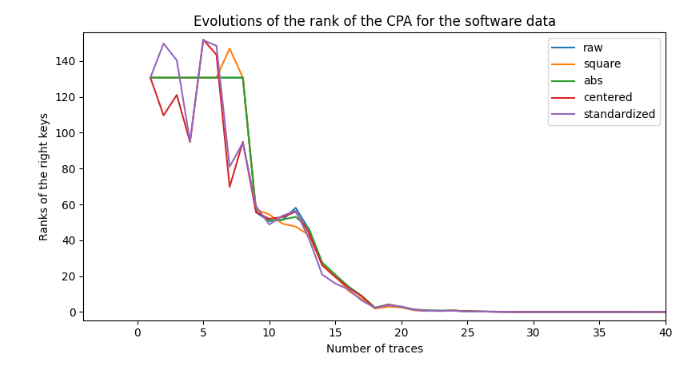
\includegraphics[width=1\linewidth]{CPA_software.png}
      \caption{CPA Rank Evolution on Software Dataset}
      \label{CPAsoftware}
    \end{subfigure}%
    \begin{subfigure}{.5\textwidth}
    \centering
      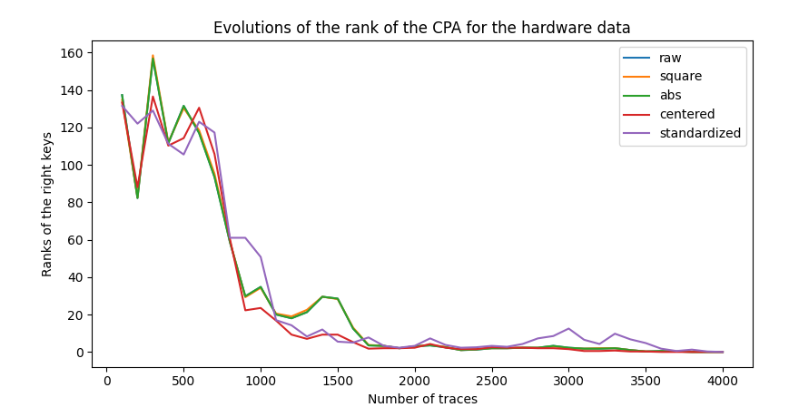
\includegraphics[width=1\linewidth]{CPA_hardware.png}
      \caption{CPA Rank Evolution on Hardware Dataset}
      \label{CPAhardware}
    \end{subfigure}
    \caption{Preprossing effects on CPA}
\end{figure}

We can see in both graphs that all preprocessing methods show a general trend where the rank of the correct key decreases as the number of traces increases. 
This indicates that more traces helps in better identifying the correct key.
\\ \\
Initially, for the software graph on the left, for the first 5-10 traces, the ranks fluctuate considerably, suggesting that with fewer traces, the CPA is less reliable regardless of the preprocessing method.
After around 10 traces, the ranks start to converge and stabilize, showing a significant improvement in identifying the correct key.
Beyond 20 traces, the ranks for all preprocessing methods approach very low values (close to 0), indicating that the correct key is being accurately identified.
\\ \\
For the hardware graph on the right, we see that in the initial phase (0-500 traces), all preprocessing methods show considerable fluctuations in the rank of the correct key, similar to the software data graph.
From around 500 to 1500 traces, all preprocessing methods show a marked decrease in the ranks, indicating an improvement in correctly identifying the key as more traces are used.
Beyond 1500 traces, the ranks for all methods converge and stabilize, generally remaining low (close to 0). This suggests that the correct key is being accurately identified with a sufficient number of traces.
\\ \\
These graphs indicate that preprocessing methods can have a some positive impact when the number of traces is low. 
However, as the number of traces increases, the impact of preprocessing diminishes, and all methods converge to effectively identify the correct key.
\subsection{LRA Rank Evolution}

\begin{figure}[h]
    \begin{subfigure}{.5\textwidth}
    \centering
      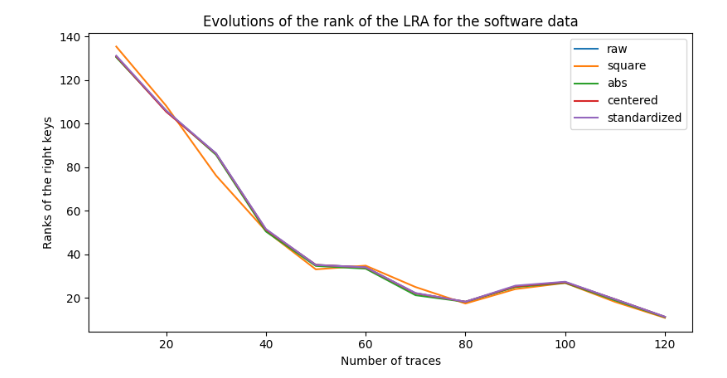
\includegraphics[width=1\linewidth]{LRA_software.png}
      \caption{LRA Rank Evolution on Software Dataset}
      \label{LRAsoftware}
    \end{subfigure}%
    \begin{subfigure}{.5\textwidth}
    \centering
      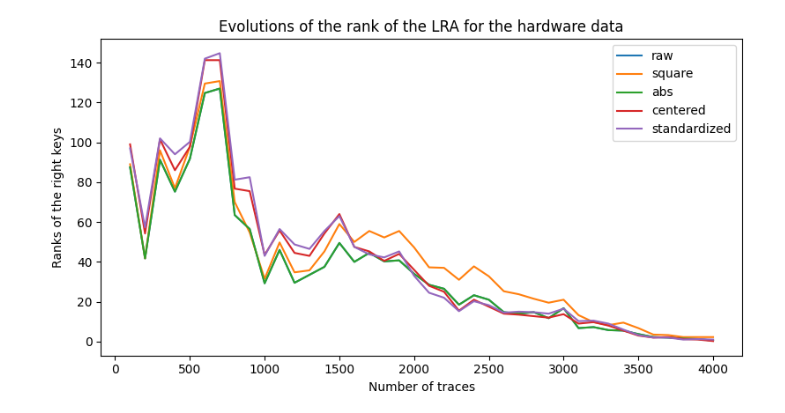
\includegraphics[width=1\linewidth]{LRA_hardware.png}
      \caption{LRA Rank Evolution on Hardware Dataset}
      \label{LRAhardware}
    \end{subfigure}
    \caption{Preprocessing effects on LRA}
\end{figure}

Similar to the CPA analysis, we see in LRA that throughout the range of traces, all preprocessing methods show very similar trends and performance.
There is no significant difference between the preprocessing methods in the context of LRA for software or hardware data as the number of traces increases. They all perform comparably well, converging to low ranks.
\newpage
\subsection{Comparison of Variability}
We can notice a high variability observed when performing CPA compared to LRA, especially on the software dataset. This can be attributed to several factors. \\ \\
CPA uses a simpler statistical model, relying on Pearson's correlation coefficient to find the relationship between power consumption and key guesses. This simplicity makes CPA more sensitive to noise and variations in the data, leading to higher variability. CPA also directly correlates power traces with hypothetical key values. If the traces have high noise or less distinct patterns, the correlation results can fluctuate significantly until sufficient traces are accumulated to stabilize the correlation.
\\ \\
On the other side, LRA models the relationship between power consumption and key guesses using linear regression, which can be more robust to noise. It considers all data points collectively, reducing the impact of outliers and variations in individual traces. Moreover, LRA involves complex matrix operations that aggregate data more effectively, smoothing out fluctuations and leading to more consistent results across different preprocessing methods.
\\ \\
The software dataset's uniformity and predictability reduce a lot the relative impact of preprocessing in LRA, while the hardware dataset's complexity and variability would make preprocessing more beneficial in improving attack effectiveness.
\section{Limitations of our Tests}
Our study had several limitations that may affect the generalizability of our results. 

\subsection{Dataset Size}
One major limitation was the size of the dataset used for testing. 
We did not analyze the entire dataset but only a small subset of traces. 
Specifically, for the software dataset, we used only 120 traces, and for the hardware dataset, we used 4000 traces. 
Moreover, these traces were not randomly selected but were the first ones available.

\subsection{Representation of Data}
This limited subset might not fully represent the variability and complexity of the entire dataset, potentially leading to biased or incomplete conclusions.
To address this, future experiments should involve:
\begin{itemize}
    \item \textit{Random Sampling}: Select traces randomly rather than sequentially to ensure a more representative sample of the dataset.
    
    \item \textit{Repeated Experiments}: Conduct multiple experiments with different randomly selected subsets of traces. Repeating the experiments multiple times would help determine if the results are consistent across different subsets and thus more reliable.
\end{itemize}

\subsection{Byte-Level Analysis}
Additionally, another important aspect to explore is the influence of preprocessing techniques at the byte level. 
It can provide deeper insights into how these techniques affect the distinguishability of key-related information. This fine-grained analysis is crucial because each byte of a cryptographic key can exhibit different leakage characteristics, and preprocessing methods may have varying effects on these individual bytes.
\\ \\
Different bytes may have different levels of susceptibility to side-channel attacks, and analyzing them individually can highlight these variances, allowing for a more nuanced approach.
\\ \\
Identifying which preprocessing techniques work best for specific bytes can help in optimizing overall attack strategies, improving the success rates of side-channel attacks.
\\ \\
Here is how we would do this byte-level analysis:\\
During the analysis, we would isolate the traces corresponding to each byte of the cryptographic key. We'd apply the various preprocessing techniques described to these isolated traces.\\
We'd measure the effectiveness of each preprocessing method on the isolated byte traces by evaluating metrics such as rank evolution.\\
Finally, we'd compare the results across different bytes to identify patterns and inconsistencies in how preprocessing techniques affect different parts of the key.

\subsection{Future Work}
By addressing these limitations in future studies, we can ensure that our results are more robust and generalizable, providing a clearer understanding of the impact of preprocessing on the success rates of side-channel attacks.

\section{Discussion}
Our investigation into the impact of preprocessing techniques on the efficacy of SCAs has 
highlighted several promising areas for future research, particularly in integrating advanced machine learning strategies such as deep learning.
The complexity and variability in SCA data make deep learning an attractive solution for uncovering and exploiting subtle vulnerabilities in cryptographic systems.

\subsection{Future Research Directions with Deep Learning}
Given the potential of deep learning to transform SCA methodologies, our future research would focus on several key areas:

\subsubsection{Enhanced Preprocessing Techniques}
Deep learning can significantly augment preprocessing stages by automating the extraction of informative features from raw side-channel measurements.
Neural networks could learn to identify and enhance signal features that are most indicative of underlying cryptographic operations, potentially surpassing traditional noise reduction and feature selection techniques.
\\ \\
Techniques such as CNNs could be utilized not just for pattern recognition but also for dynamically adjusting the preprocessing steps based on the observed data characteristics.
\\ \\
Research by Kwon, Kim, and Hong on using autoencoders for non-profiled deep learning-based side-channel preprocessing exemplifies the potential benefits of integrating deep learning into preprocessing stages \cite{9400816}.
\\ \\ 
Integrating deep learning into existing SCA frameworks can lead to a hybrid approach where deep learning aids in refining the 
preprocessing steps for traditional methods like CPA and LRA. 
For example, a deep learning model could initially process the raw traces to enhance or highlight features that are then fed into CPA or LRA analyses.

\section{Conclusion}
Our research has delved into the impact of preprocessing techniques on the effectiveness of side-channel attacks, specifically focusing on Correlation Power Analysis and Linear Regression Analysis applied to power traces from both software and hardware implementations of the AES algorithm. Through our study, several key insights emerged. \\ \\
Our findings indicate that preprocessing methods such as raw, squared, absolute value, centered, and standardized traces do not significantly enhance the effectiveness of CPA and LRA in most scenarios. As the number of traces increases, the influence of preprocessing diminishes, and all methods tend to converge towards accurate key identification. \\ \\
CPA exhibited higher variability in results compared to LRA. This is due to CPA's reliance on Pearson's correlation coefficient, making it more sensitive to noise and variations in the data. LRA, with its robust modeling through linear regression, aggregates data more effectively, leading to consistent results across different preprocessing methods. \\ \\
Our study was limited by the size of the datasets used. We analyzed only small subsets of traces, which may not fully represent the variability and complexity of the entire datasets. Future studies should incorporate random sampling and repeated experiments to ensure more robust and generalizable results. Additionally, analyzing the influence of preprocessing at the byte level could provide deeper insights into improving SCA success rates. \\ \\
The integration of advanced machine learning techniques, such as deep learning, holds promise for enhancing preprocessing stages. \\ \\
In conclusion, while preprocessing shows limited effectiveness in larger datasets, it remains a crucial area for improving side-channel attack strategies. Further exploration and experimentation are necessary to fully harness the potential of these advanced techniques in the context of side-channel analysis. Our study lays the groundwork for future research aimed at refining SCA methodologies and improving cybersecurity measures.

\bibliography{ResearchPaperBib}

\end{document}
